\documentclass[12pt]{article}

% Font family
\usepackage{xeCJK}
\setCJKmainfont{Noto Serif TC}
\usepackage{amssymb}
\usepackage{amsmath}

% Document layout
\usepackage[margin=2cm, a4paper]{geometry}
\usepackage{setspace}
\onehalfspacing
\setlength{\parskip}{12pt}
\setlength{\parindent}{0pt}

% Citation
\usepackage{biblatex}
\addbibresource{./ref.bib}

% Image
\usepackage{graphicx}
\graphicspath{{./images/}}

\author{\normalsize 施宇庭 NN6124030}
\date{}


\title{\Large AOC 2024 Spring - Lab 4 Processing Element}

\begin{document}
\maketitle

\section{Implmenetation of Eyeriss PE}
% (15% / 15% / 15%) 1. Pass all testbenches. Screenshots of passing 3 tbs.
% (10%) 2. Cycle comparison of each tb. Each tb contains 3 points.

% \subsection*{Testbench 0 Passed}
\begin{figure}[h]
    \centering
    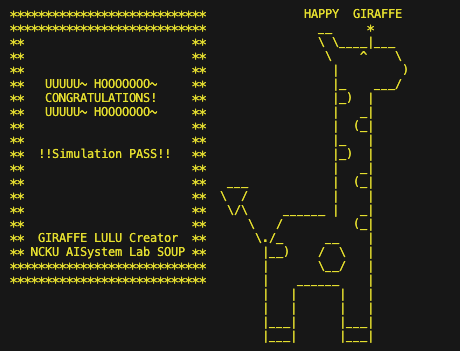
\includegraphics[width=0.35\linewidth]{tb0.png}
    \caption{Testbench 0 Passed}
\end{figure}

% \subsection*{Testbench 1 Passed}
\begin{figure}[h]
    \centering
    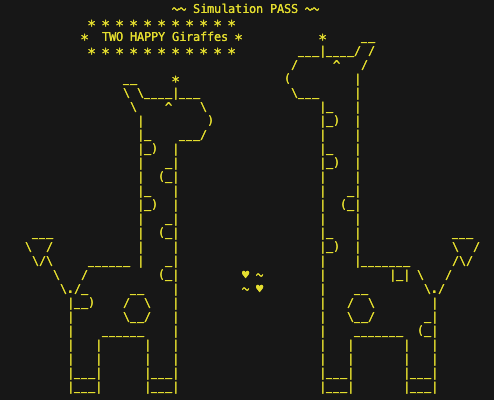
\includegraphics[width=0.35\linewidth]{tb1.png}
    \caption{Testbench 1 Passed}
\end{figure}

% \subsection*{Testbench 2 Passed}
\begin{figure}[h]
    \centering
    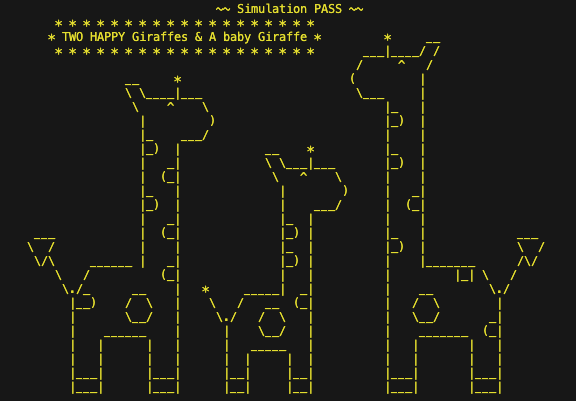
\includegraphics[width=0.35\linewidth]{tb2.png}
    \caption{Testbench 2 Passed}
\end{figure}

\section{PE Design}
% (20%) 3. Draw your own PE architecture.
% Write down your total spad storage space and the corresponding functions.
% Explain how your PE works with waveform clearly. Mark down the values you mention.

\subsection*{Architecture}
\begin{figure}[h]
    \centering
    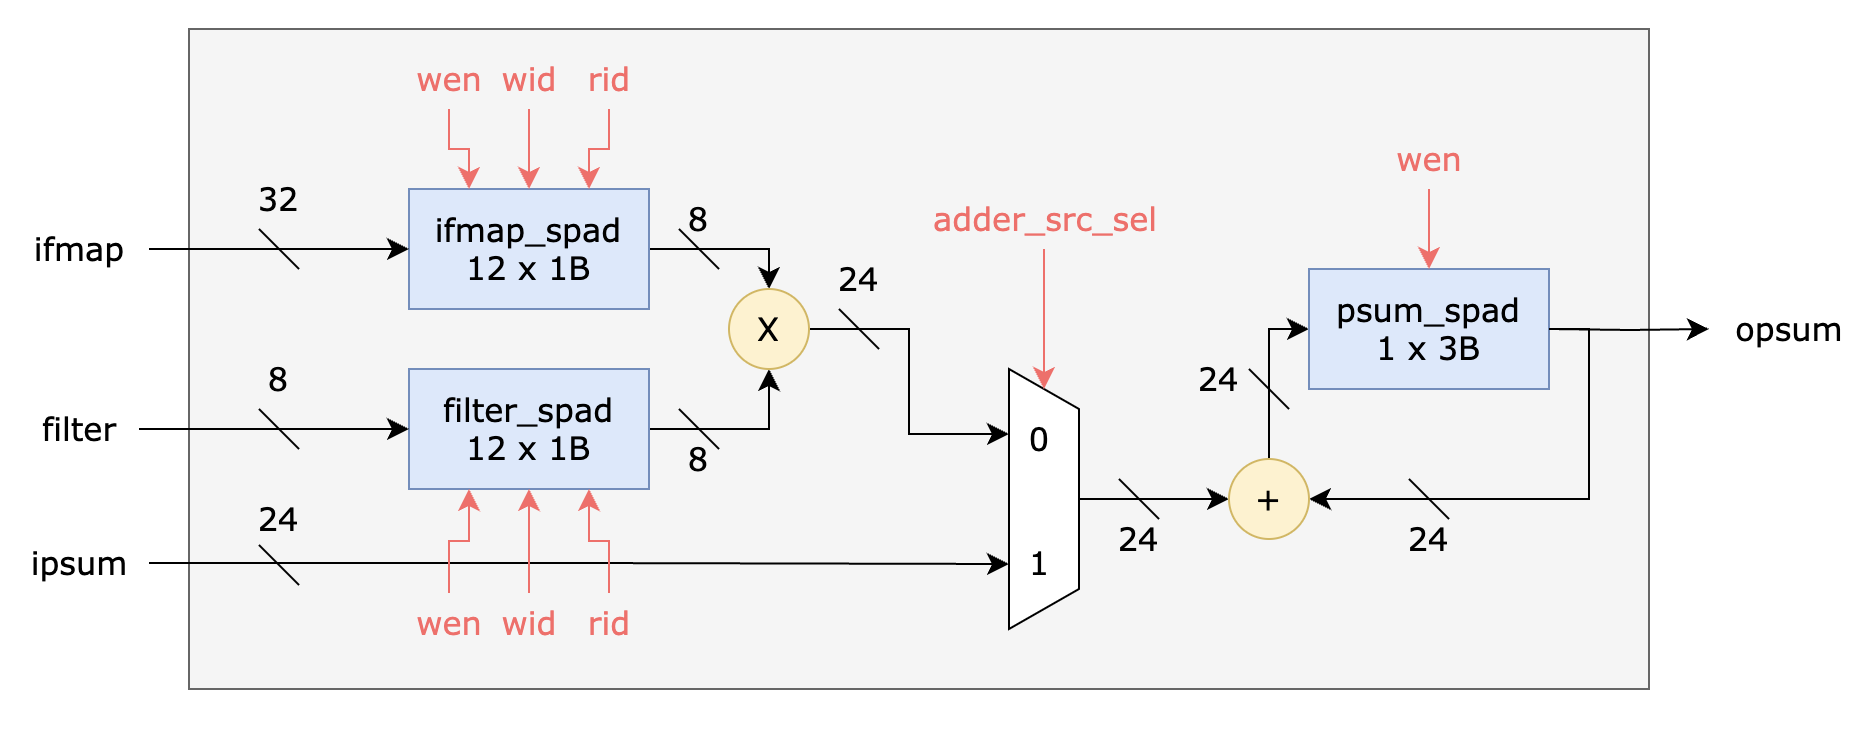
\includegraphics[width=0.7\textwidth]{arch.png}
    \caption{Hardware architecture of Eyeriss PE.}
    \label{fig:arch}
\end{figure}

\subsection*{State Transition}
\begin{figure}[h]
    \centering
    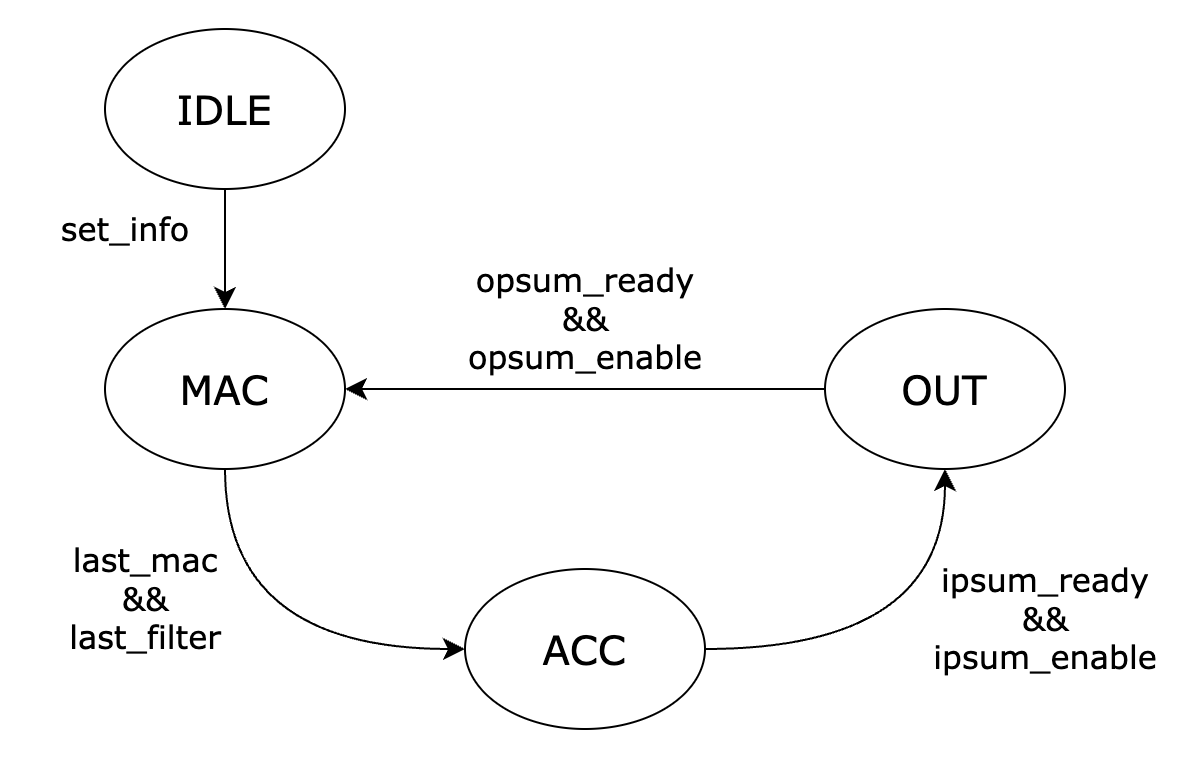
\includegraphics[width=0.5\textwidth]{fsm.png}
    \caption{Finite state machine of PE controller.}
    \label{fig:fsm}
\end{figure}

\subsection*{Control Signals}
\begin{table}[h]
    \begin{tabular}{|l|lll|lll|l|l|}
    \hline
         & \multicolumn{3}{l|}{ifmap}                                       & \multicolumn{3}{l|}{filter}                                      & adder    & psum \\ \hline
         & \multicolumn{1}{l|}{wen} & \multicolumn{1}{l|}{wid}        & rid & \multicolumn{1}{l|}{wen} & \multicolumn{1}{l|}{wid}        & rid & src\_sel & wen  \\ \hline
    IDLE & \multicolumn{1}{l|}{0}   & \multicolumn{1}{l|}{0}          & 0   & \multicolumn{1}{l|}{0}   & \multicolumn{1}{l|}{0}          & 0   & DC       & 0    \\ \hline
    MAC &
      \multicolumn{1}{l|}{1} &
      \multicolumn{1}{l|}{\textless{}oldval\textgreater + 4} &
      \textless{}old\_val\textgreater +1 &
      \multicolumn{1}{l|}{1} &
      \multicolumn{1}{l|}{\textless{}oldval\textgreater + 1} &
      \textless{}oldval\textgreater +1 &
      0 &
      1 \\ \hline
    ACC  & \multicolumn{1}{l|}{0}   & \multicolumn{1}{l|}{DC}         & DC  & \multicolumn{1}{l|}{0}   & \multicolumn{1}{l|}{DC}         & DC  & 1        & 1    \\ \hline
    OUT  & \multicolumn{1}{l|}{1}   & \multicolumn{1}{l|}{0 if clear} & 0   & \multicolumn{1}{l|}{1}   & \multicolumn{1}{l|}{0 if clear} & 0   & DC       & 0    \\ \hline
    \end{tabular}
    \caption{Control signals of PE controller.}
\end{table}

\section{Row Stationary Dataflow with Ifmap Reuse}
% (10%) 4. Demonstrate Scenario B dataflow by completing 2 3row x 3col x 2ch ofmaps
% by 2-channel of 2 3x3 filters(kernel) and 2 5x5 ifmaps under parameters n=1, p=2(kernel),
% q=1(channel).

\begin{table}[h]
    \centering
    \begin{tabular}{c|cccc}
    \hline
           & batch size & channels & height & width \\ \hline
    filter & 2          &  2       & 3      & 3     \\ \hline
    ifmap  & 2          &  2       & 5      & 5     \\ \hline
    ofmap  & 2          &  2       & 3      & 3     \\ \hline
    \end{tabular}
    \caption{Convolution 2D shape parameters.}
\end{table}

\begin{figure}[h]
    \centering
    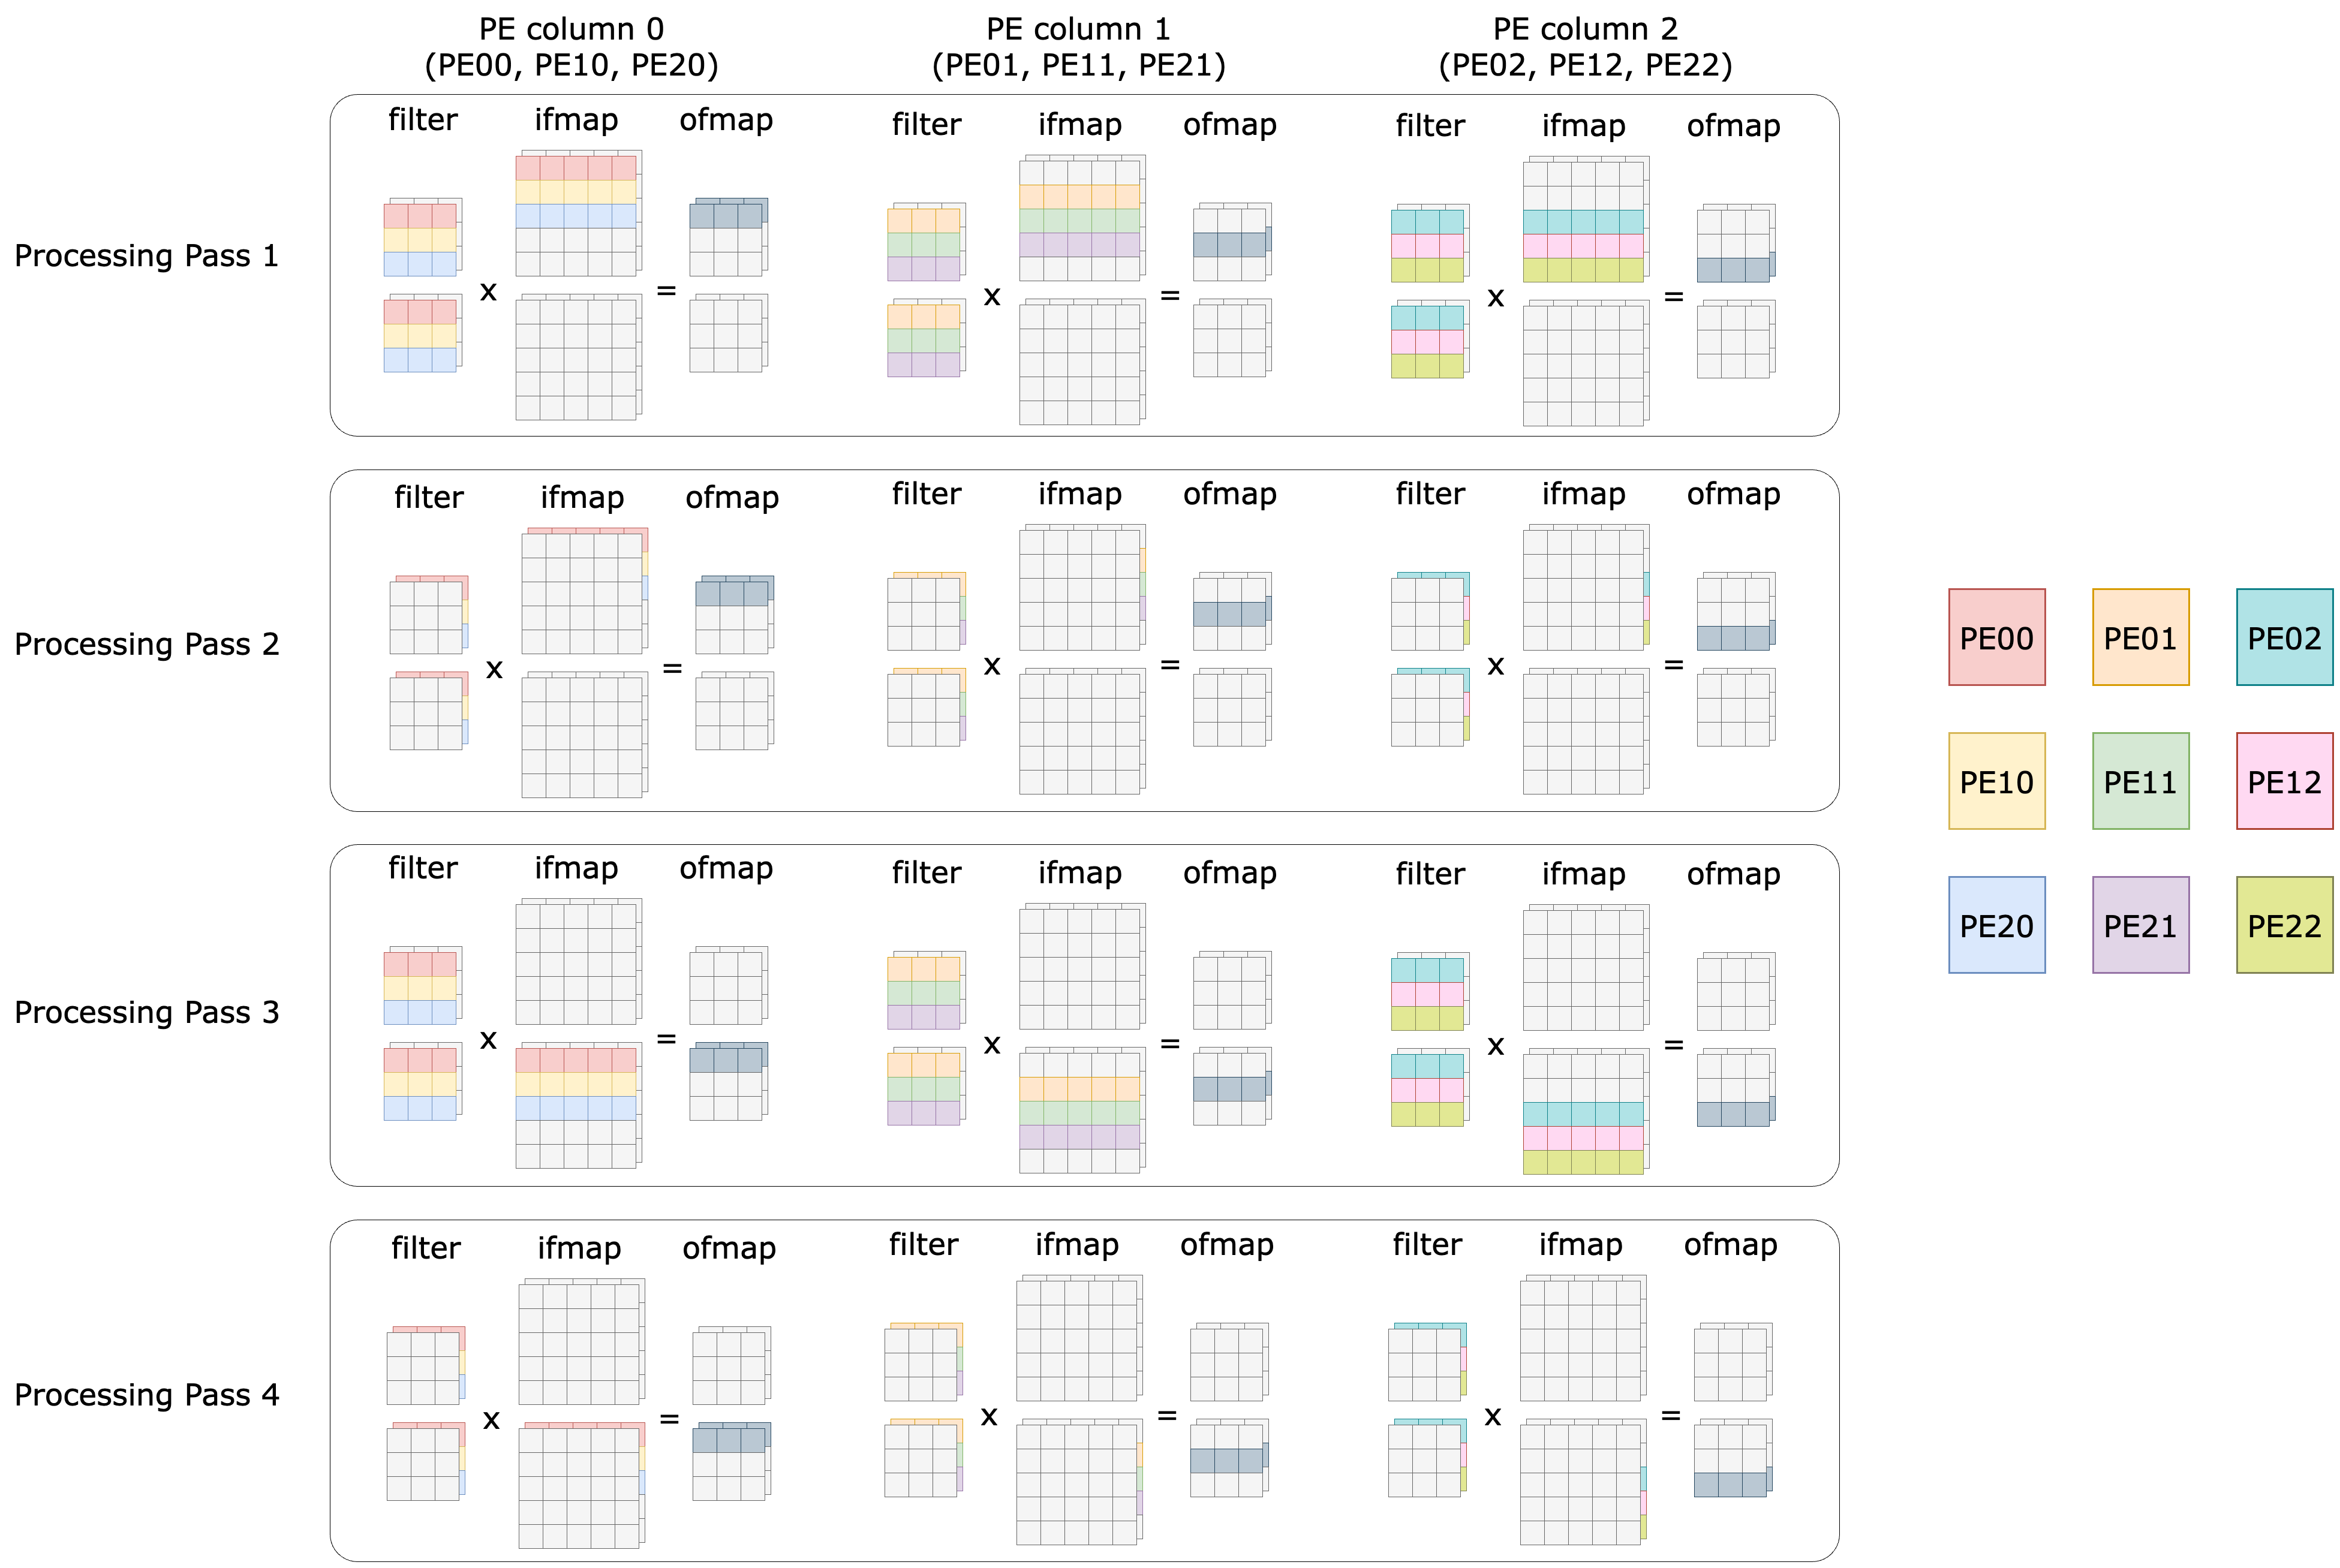
\includegraphics[width=\linewidth]{dataflow.png}
    \caption{Processing passes and workload mapping of row stationary dataflow with ifmap reuse.}
    \label{fig:mul_arch2}
\end{figure}
\newpage

\section{Comparison of Row Stationary Dataflow in Different Scenarios}
% (10%) 5. Compare scenario A,B,C from different aspects organized into a table.
% Analyze under scenario A(n=2, p=1, q=1), scenario B(n=1, p=2, q=1), scenario C(n=1, p=1,
% q=2) within a processing pass and across multiple passes to complete 2 3row x 3col x 2ch
% ofmaps by 2-channel of 2 3x3 filters(kernel) and 2 5x5 ifmaps.
% (Hint : reuse distances of ifmap, filter and psum(lec4 p.116-126), proper spad size in a PE,
% numbers of memory read / write of ifmap, filter and psum and energy consumption (lec4 p.146、lec5 p.60-67), pros and cons etc.)

\begin{table}[h]
    \centering
    \begin{tabular}{|c|c|c|c|}
    \hline
        & filter reuse (A) & ifmap reuse (B) & psum reuse (C) \\ \hline
    n   &     2            &        1        &      1          \\ \hline
    p   &   1              &        2        &      1          \\ \hline
    q   &      1           &        1        &      2          \\ \hline
    \end{tabular}
    \caption{RS dataflow mapping prameters of filter reuse (scenario A), ifmap reuse (scenario B), and psum reuse (scenario C).}
\end{table}

\begin{figure}
    \centering
    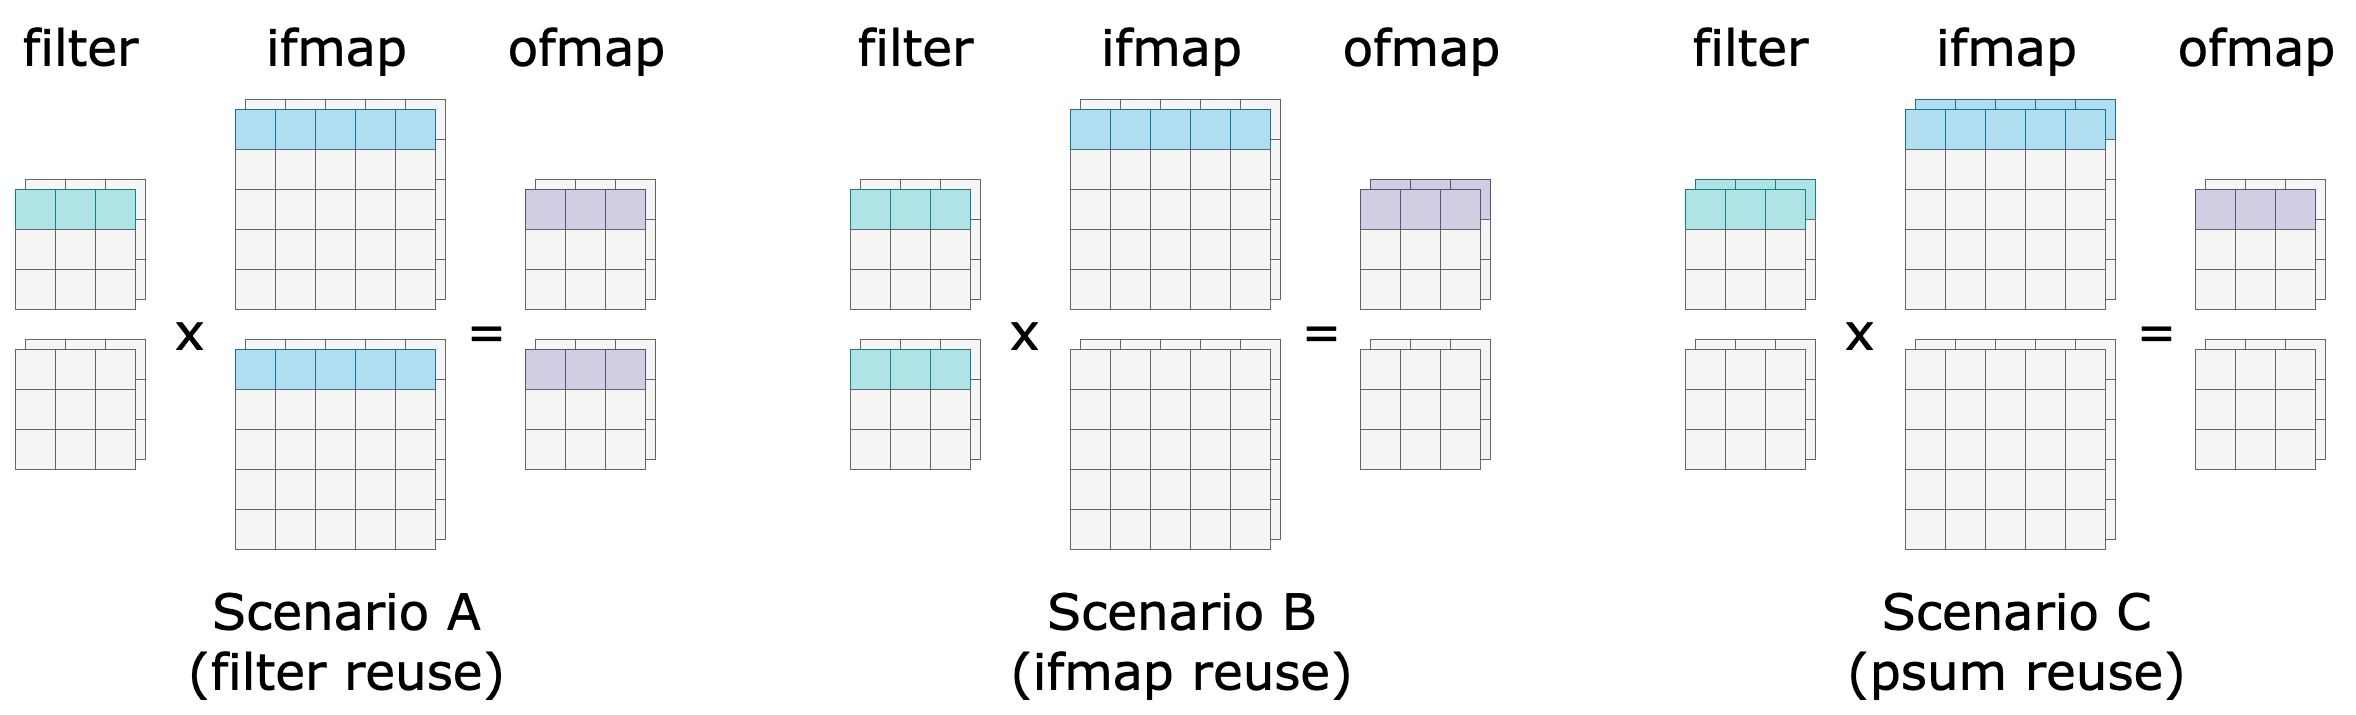
\includegraphics[width=0.8\linewidth]{reuse.png}
    \caption{Schematic diagram of row stationary dataflow in different scenarios.}
\end{figure}

\begin{table}[h]
    \centering
    \begin{tabular}{|c|c|c|c|}
    \hline
                                                                                   & filter reuse (A) & ifmap reuse (B) & psum reuse (C) \\ \hline
    \begin{tabular}[c]{@{}c@{}}reuse distance\\ (filter/ifmap/psum)\end{tabular}   & 1/4/2       &   6/1/2   &    6/4/1      \\ \hline
    \begin{tabular}[c]{@{}c@{}}proper spad size\\ (filter/ifmap/psum)\end{tabular} & 3/6/2        &   6/3/2     & 6/6/1       \\ \hline
    % \begin{tabular}[c]{@{}c@{}}num of mem read\\ (filter/ifmap/psum)\end{tabular}  &              &             &             \\ \hline
    % \begin{tabular}[c]{@{}c@{}}num of mem write\\ (filter/ifmap/psum)\end{tabular} &              &             &             \\ \hline
    % energy consumption                                                             &              &             &             \\ \hline
    % pros                                                                           &              &             &             \\ \hline
    % cons                                                                           &              &             &             \\ \hline
    \end{tabular}
    \caption{Comparison of reuse distance, proper spad size, number of memory read/write and energy consumption between 3 scenarios.}
\end{table}

\pagebreak

\section{Thoughts and Advices}
% (5%) 6. Share your thoughts on this lab. Any takeaways or advices?

\begin{itemize}
    \item lab 的講解可以簡潔一點,講義和影片都太過冗長不易抓到重點
    \item testbench 有些行為並沒有在規格中說明清楚,例如 overflow handling、timing spec 等等
    \item 講義中可以不用放不相關的內容
\end{itemize}

\section{Improvement of PE Design}
% (Bonus 20%) 7. (15%) Modify your PE to a pipelined architecture or with zero-gating / zero
% skipping function. You can choose one from 3 functions to implement.

這次的 PE 設計當中我採用了以下兩種方式來改進 PE 的運算效率:
\begin{enumerate}
    \item zero-skipping:PE 可以支援 channel = \{1, 2, 3, 4\},當 channel size 較小時,可以跳過部分 MAC 運算
    \item asynchronous data fetching:不需要等到 ifmap 和 filter 全部拿完才開始進行運算,MAC computation 和 data fetching 由不同的 FSM 來控制,因此可以獨立進行
\end{enumerate}

% \section{Comparison between PE Architectures}
% (5%) Theoretically compare with basic PE architecture on page 33, 58 by required cycles,
% effectual and ineffectual operations(lec4 p.16-19、25), etc.

\end{document}
